\documentclass[../main]{subfiles}
\begin{document}

\newcommand{\refsec}[1]{
  \begin{tikzpicture}
  \node[rounded corners,fill=red] (0,0) {#1};
\end{tikzpicture}
}




\section{Konventionen und Notation}

\subsection*{Beschriftung}

\begin{tabular}{ll}
  $\vec{v}$ & ein Vektor \refsec{Test} \\
  $\mat{M}$ & eine Matrix \\
  $\trs{\mat{M}}$ & eine transponierte Matrix \\

\end{tabular}


\subsection*{Konventionen}

\begin{itemize}

\item{
    Falls ein (Zeilen- oder Spalten-) Vektor $\vec{v}$ als Argument in eine
    Funktion $f$ gegeben wird, bedeutet dies,
    dass die einzelnen Komponenten des Vektors die Parameter der Funktion sind.
    \begin{equation*}
      f(\vec{v})=f(v_1,\ldots,v_n)
    \end{equation*}
  }

\item{
    Falls die Klammern, in denen der Vektor $\vec{v}$ steht, als eckige
    Klammern [] geschrieben sind, bedeutet dies, dass es sich um die
    Vektorisierung einer Funktion $f$ handelt, somit wird die Funktion auf
    jede Vektorkomponente angewandt.
    \begin{equation*}
      f[\vec{v}]=
      \begin{pmatrix}
        f(v_1)\\
        \vdots \\
        f(v_n)\\
      \end{pmatrix}
    \end{equation*}
  }

\end{itemize}

ERWEITERN


\pagebreak
\section{Machinelles Lernen - Theorie}

Der Themenbereich des \textbf{Machinellen Lernens} beschäftigt sich mit Algorithmen und mathematischen Modellen, welche von selber lernen, Probleme zu loesen.
Hierzu werden keine expliziten Instruktionen fest einprogrammiert (engl.:\ hard coding), sondern das Modell wird trainiert und optimiert sich von selbst.
Dabei wird das Modell mit Trainingsdaten befuettert, mithilfe eine Korrelation zwischen den Inputdaten und den Outputdaten erlernt werden soll.
Der Zusammenhang der Daten wird von den Modellen verallgemeinert und das Modell kann dann Vorhersagen fuer neue Daten machen.

\subsection{Allgemeine Begriffe}

\subsubsection{Daten}

Der \textbf{Trainingsdatensatz} $\mathbb{T}$ beinhaltet gewisse \textbf{Attribute}, die Merkmalstypen der Inputdaten.
Die \textbf{Features} sind dann die spezifischen Werte der Attribute eines Trainingssample.
Die sogenannten \textbf{Labels} sind die erwarteten Outputs, welche der Algorithmus vorherzusagen hat.
Diese Vorhersagen werden mit den Labels abgeglichen und so bewertet.
Anhand der Bewertungen wird dann eine Optimierung des Modells vorgenommen.
Unter korrekten Bedingungen (keine Ueberanpassung) findet kein Auswendiglernen der Trainingsdaten statt,
sondern ein Generalisieren des Zusammenhangs anhand von Mustern und Gesetzmassigkeiten.
\par\medskip
Um eine endgueltige Bewertung des Modells durchzufuehren, wird ein Testdatensatz, welcher nicht Teil des Trainingsdatensatz ist, genutzt um Vorhersagen zu machen.
Dies garantiert, dass kein Auswendiglernen moeglich ist.
\par\medskip
Die Inputs/Features werden in einem Vektor $\vec{x}=\trs{(x_1,x_2,\ldots,x_n)}$ und die Outputs/Vohersagen in einem Vektor $\vec{y}=\trs{(y_1,y_2,\ldots,y_m)}$ zusammengefasst.
Das gleiche macht man mit den Labels, wobei diese mit $\vec{\hat{y}}=\trs{(\hat{y}_1,\hat{y_2},\ldots,\hat{y}_m)}$ bezeichnet werden.
\par \medskip
BESSERS BEISPIEL -> UM SPAETER KONKRETES MODELL ZU ERKLAEREN
Am Beispiel eines Datensatz, welcher fuer Bilderkennung von Hunden und Katzen genutzt wird, werden diese Begriffe verdeutlicht.
Die Inputdaten sind die Fotos von Hunden und Katzen. Deren Attribute sind die moeglichen RGB-Farbenwerte (drei Zahlen, welche von 0 bis 255 reichen) aller Pixel.
Die Features sind die spezifischen RGB-Werte der Pixel fuer die einzelnen Bilder. Die Outputdaten sind die Labels, welche in diesem Fall angeben, ob ein Hund oder eine Katze auf dem Bild gezeigt wird.
Dies wird meistens mit einer One-Hot-Kodierung bzw.\ einem One-Hot-Vektor
gemacht. Jeder Labelart wird eine eigene Vektorkomponente zugewiesen. Falls das
Label aktiv ist, ist die Komponent 1 ansonsten 0. Somit kann Hund als $\vec{l}_H={(1,0)}^T$ reprasentiert werden und Katze als $\vec{l}_K={(0,1)}^T$.

\begin{figure}[h!]
  \centering
  \begin{tikzpicture}[node distance=5cm,auto]

  \end{tikzpicture}

  \caption{eine Veranschaulichung des beschriebenen Machine Learning Modells}
\end{figure}

\subsubsection{Modelle}
Ein \textbf{Modell} ist eine mathematische Funktion $\mathit{f}\colon \mathbb{R}^n \to \mathbb{R}^m$, welche die Inputs auf die Outputs abbildet $\vec{y}=\mathit{f}(\vec{x})$.
Im Zusammenhang mit Wertevorhersagen spricht man von einem Regressionsmodell.
Das Verhalten dieses Modells wird bestimmt durch seine \textbf{Modellparameter} $\phi_1, \phi_2,\ldots$.
Das Ziel ist es, die Modellparameter so einzustellen, dass die Vorhersagen $\vec{y}$ besser mit den Labels $\vec{\hat{y}}$ uebereinstimmen.
Dies wird iterativ gemacht, indem immer wieder leichte Anpassungen an den Parametern vorgenommen werden, bis sie das gewuenschte Resultat liefern.
\par\medskip
Das wohl einfachste Regressionsmodell ist eine Regressionsgerade. Diese ist
angemessen, falls ein einfacher linearen Zusammenhang der Form $y=\phi_1x +
\phi_0$ zwischen den Features und den Labels besteht.
Nun muessten nur noch $\phi_0$ und $\phi_1$ bestimmt werden.

Neben den gelernten Parametern, gibt es auch noch sogenannte \textbf{Hyperparameter}.
Diese koennen nicht erlernt werden, sondern muessen manuell vor dem Training gewaehlt werden und koennen den Lernvorgang erheblich beeinflussen.
\par\medskip
Fuer Machine Learning haben sich gewisse Modelle besonders guet etabliert,
darunter waeren: Support Vector Machines, Evolutionäre Algorithmen, und Künstliche Neuronale Netze.
Diese Arbeit wird sich vorwiegend mit Neuronalen Netzen auseinandersetzen.
\par\medskip
BEISPIELMODELL GLEICHES WIE VORHIN
% Um den Modellbegriff noch etwas zu festigen wird ein Beispielmodell erlautert:\\
% Das Modell soll Vorhersagen zum Wetter machen. Anhand von Luftfeuchtigkeit und
% Temperatur muss es eine Aussage treffen, ob es gerade regnet oder nicht.

\begin{figure}[h!]
  \centering

  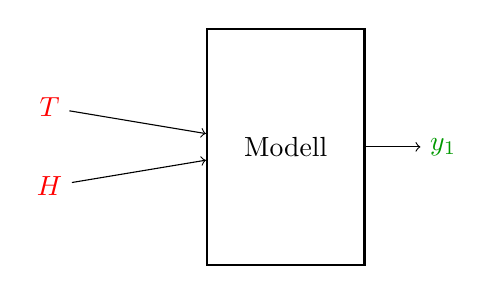
\begin{tikzpicture}
    \path (3,0) node [draw,thick,minimum width=2cm,minimum height=3cm](neuron){Modell};
    \path[red] (0,0.5) node(T){$T$} (0,-0.5) node(H){$H$};
    \path[black!40!green] (5,0) node(y1){$y_1$};
    \draw[->] (T) -- (neuron);
    \draw[->] (H) -- (neuron);
    \draw[->] (neuron) -- (y1);

  \end{tikzpicture}

  \caption{Darstellung eines Modells}
\end{figure}

\subsection{Training}
\subsubsection{Kostenfunktionen}
Einsicht ist der erste Schritt zur Besserung. Das gilt auch beim Machine Learning, deshalb muss beim Training zuerst die Genauigkeit des Modells bewertet werden.
Dafuer gibt es sogennante \textbf{Kosten-, Verlust- oder Fehlerfunktionen}. Sie sollen ein Mass fuer die Abweichung des Outputs $\vec{y}$ vom Label $\vec{\hat{y}}$ sein.
\par\medskip
Die Fehler der einzelnen Outputs $c(y_i,\hat{y}_i)$ werden aufsummiert um den
Fehler $C(\vec{y}_j,\vec{\hat{y}}_j)$ (wobei $\vec{y}_j$ die Vorhersagen sind und
$\vec{\hat{y}}_j$ die Labels sind) einer gesamten Vorhersage zu berechnen. Siehe Gleichung (\ref{eq:errorfunc}).\\
Der Fehler $\bar{C}(\mathbb{T})$ eines ganzen Datensatzes $\mathbb{T}$, der
Groesse $p$ ergibt sich aus dem arithmetischen
Mittel der einzelnen Vorhersagen-Fehler. Siehe Gleichung (\ref{eq:meanerrorfunc}).
\par\medskip
\begin{minipage}[h!]{0.5\textwidth}
  \centering
  \begin{equation}\label{eq:errorfunc}
    C \left(\vec{y},\vec{\hat{y}} \right)=\displaystyle\sum_{i=1}^{m} c(y_i, \hat{y}_i)
  \end{equation}
\end{minipage}
\begin{minipage}[h!]{0.5\textwidth}
  \centering
  \begin{equation}\label{eq:meanerrorfunc}
    \bar{C}(\mathbb{T}) = \frac{1}{p}\displaystyle\sum_{j=1}^{p} C\left(\vec{y}_j,\vec{\hat{y}}_j\right)
  \end{equation}
\end{minipage}
\par\medskip
Eine Kostenfunktion sollte folgende Eigenschaften aufweisen:
\begin{itemize}
\item{$c$ ist minimal, wenn $y = \hat{y}$}
\item{$c$ waechst mit $|\vec{y}-\vec{\hat{y}}|$}
\item{$C$ ist nach jedem $y_n$ partiell differenzierbar (erklaert in Sektion (\ref{sec:partielle_ableitungen}))}
\end{itemize}

Eine beliebte Kostenfunktion ist die ``Mittlere quadratische Abweichung'' (engl.:\ mean squared error).\\
$\displaystyle C_{MSE} = \frac{1}{2n}\sum_{i=1}^{n}{(\hat{y}_i - y_i)}^2 = \frac{1}{2n}{(\vec{\hat{y}} - \vec{y})}^2$.
Sie erfuellt alle anforderungen, denn:
Sie ist $0$ falls $y=\hat{y}$. Sie ist proportional zu ${(\hat{y}-y)}^2$ und ihre Ableitung nach $y$ lautet: $C'=\frac{1}{n}(y-\hat{y})$


\subsubsection{Gradientenverfahren}
Um ein Modell nun zu trainieren, muss man verstehen, dass es sich um ein Optimierungsproblem handelt.
Das Modell ist am besten, also macht die besten Vorraussagen, wenn die
Funktionswerte der Fehlerfunktion am kleinsten sind.
Deshalb muss diese Fehlerfunktion $C$ minimiert werden.
Hierbei muss die Funktion $C$ nicht mehr in Abhaengigkeit der Inputs betrachtet werden, sondern in Abhaengigkeit von den Modellparametern
$C(\phi_1, \phi_2, \ldots, \phi_n)$, denn diese sollen angepasst werden, um das Modell zu verbessern.
Fuer diese Optimiertung wird das sogennante \textbf{Gradientenverfahren} (engl.: Gradient descent) verwendet.
\footnote{
  Im Gymnasium wird beigebracht die lokalen Extrema (inkl.\ lokalen Minimas) zu bestimmen, indem die erste Ableitung $f'$ gebildet wird und  gleich null gesetzt wird.
  Dies ist hier nicht moeglich, da die Funktion $C'(\phi_1,\phi_2, \ldots, \phi_n)$ deutlich zu komplex ist, um die Nullstellen zu bestimmen. Deshalb wird das Gradientenverfahren verwendet.
}
\par\medskip
Allgemein koennen mithilfe des Gradientenverfahrens Funkionen $f(x_1, x_2, \ldots, x_n)$ vom Typ $\mathbb{R}^n \to \mathbb{R}$ (wie z.B. die Fehlerfunktion) minimiert werden.
Dies geschieht, indem ein Startpunkt (Ortsvektor) $\vec{p}_0$, dessen Komponenten den Input von $f$ darstellt, gewaehlt wird.
Nun werden iterativ neue Punkte $\vec{p_z}$ gesucht, welche immer naeher beim lokalen Minimun liegen, also Punkte, die den Funktionswert $f(\vec{p}_z)$ immer kleiner werden lassen.
Dies wird durchgeführt, bis der Punkt genug nahe beim lokalen Minimun ist.
\par\medskip
Dafuer muss ein Vektor $\vec{b}_z$ bestimmt werden, welcher auf den Punkt $\vec{p}_z$ draufaddiert einen neuen Punkt $\vec{p}_{z+1}$ bildet,
bei dem der Funktionswert $f(\vec{p}_{z+1})$ kleiner ist als der von $f(\vec{p}_z)$.
Dies geschieht am effizientesten, wenn $\vec{b}_z$ in die Richtung der staerksten Funktionswertabnahme zeigt.

Hierzu braucht man den sogennanten \textbf{Gradient} $\vec{\nabla}$, wofür man wiederum partielle Ableitungen braucht.
\par\medskip

\begin{defbox}{Partielle Ableitungen}
  Partielle Ableitungen sind eine Erweiterung der ``normalen'' Ableitungen auf multidimensionale Funktionen $f(x_1,\cdots,x_n)$.
  Man leitet dabei nur nach einem Parameter $x_i$ ab und betrachtet die restlichen Argumente als Konstanten.
  Es gelten die gleichen Ableitungsregeln wie bei der nicht-partiellen Ableitung.
  Die partielle Ableitung einer Funktion $f(x_1,\cdots,x_n)$ bezueglich der Variable $x_i$ in einem Punkt $\vec{a}=(a_1,\cdots,a_n)^T$ ist analog zur ``normalen'' Ableitung folgendermassen definiert:
  \begin{equation*}
    \frac{\partial f}{\partial x_i}(\vec{a}) \coloneqq \lim_{h \to 0} \frac{f(a_1,\cdots,a_i + h,\cdots,a_n)-f(a_1,\cdots,a_i,\cdots,a_n)}{h}
  \end{equation*}
  Geometisch ist dies die Steigung der Tangente im Punkt $\vec{a}$ in Richtung der Achse des Parametern $x_i$, nach dem man ableitet.
\end{defbox}
    
\par\medskip

\begin{defbox}{Gradient}
  Der Gradient $\vec{\nabla}$ ist ein Differentialoperator, welcher ein Skalarfeld auf ein Vektorfeld (das sogennante Gradientenfeld) abbildet.\\
  Dabei fasst man alle partiellen Ableitungen einer Funktion $f$ in einem Vektor zusammen.
  \begin{equation*}
    \vec{\nabla}f=
    \begin{pmatrix}
      \frac{\partial f}{\partial x_1} \\
      \vdots \\
      \frac{\partial f}{\partial x_n} \\
    \end{pmatrix}
  \end{equation*}
  Geometisch ist der Gradient $\vec{\nabla}f(\vec{p})$ einer Funktion $f$ in einem Punkt $\vec{p}$ dann der Vektor, welcher in die Richtung des steilsten Anstiegs von $f$ zeigt.
  Sein Betrag gibt die Staerke des Anstiegs an.
\end{defbox}

Da der Gradient in die Richtung des steilsten Anstiegs zeigt, sollte der Vektor $\vec{b}_z$ in die Richtung des negierten Gradient der Funktion $f$ im Punkt $\vec{p}_z$ zeigen.
Also kann jetzt das iterative Annahern an das lokalen Minimums so beschrieben
werden (wobei $\eta$ eine spaeter erklaerte Schrittgroesse darstellt):\\
\begin{equation}\label{eq:gradientdescent}
  \vec{p}_{z+1} = \vec{p}_z - \eta \cdot \vec{\nabla} \mathit{f}(\vec{p}_z)
\end{equation}

BEISPIEL FUER GRADIENTENVERFAHREN MIT ABBILDUNG

\begin{figure}[h!]
  \centering

  \caption{Darstellung des Gradientenabstiegs}
\end{figure}

Waehrend des Gradientenverfahren konvergiert der Punkt $\vec{p}_z$ zu einem belibigen \textit{lokalen} Minimum, abhängig davon wie der Startpunkt $\vec{p}_0$ gewaehlt wurde.
Da dieser meist zufaellig bestimmt wird, ist es eine Glückssache ein sehr niedriges Minimum zu finden.
\par\medskip
Die sogennante \textbf{Lernrate} $\eta$ aus Gleichung (\ref{eq:gradientdescent}) ist ein Hyperparameter.
Sie ist ein positiver Proportionalitatsfaktor, welcher die Schrittgroesse des Gradientenabstieg bestimmt. Sie muss je nach zu minimierender Funktion anderst gewaehlt werden.
Dabei hilft nur ausporbieren. Falls $\eta$ nicht gut gewahelt wurde, gibt es Probleme beim Training:
\begin{itemize}
\item{Falls $\eta$ zu klein ist, verlaueft das Trainings unnotig langsam und braucht sehr lange.
    Ausserdem kann es passieren, dass man bei einem hohen lokalen Minimum stecken bleibt.}

\item{Falls $\eta$ zu gross ist, passiert es, dass man ueber das lokale Minimum hinaus schiesst und nur darum herum springt.}
\end{itemize}

\begin{figure}[h!]
  \centering
  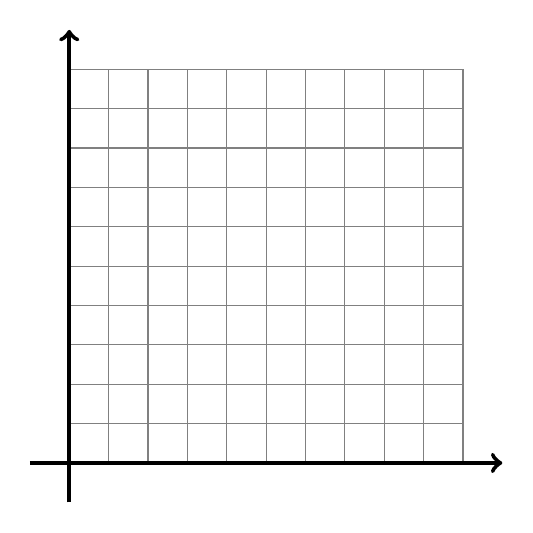
\begin{tikzpicture}
    \draw[gray] (0,0) grid[step=0.5cm] (5,5);
    \draw[ultra thick,black,->] (-0.5,0) -- (5.5,0);
    \draw[ultra thick,black,->] (0,-0.5) -- (0,5.5);

  \end{tikzpicture}
  \caption{Visualiesierung verschiedener Lernraten}
\end{figure}

\subsubsection{Stochastisches Gradientenverfahren fuer Machine Learning}
Wie vorhin erklaert, wird fuer das Trainieren eines Modells das Gradientenverfahren benutzt.
Konkret wird die Kostenfunktion $C(\vec{y},\vec{\hat{y}}|\phi_0,\ldots,\phi_n)$
($\phi$ sind die Modellparameter, $\vec{y}$ die Vorhersagen und $\vec{\hat{y}}$
die Labels) minimieren, indem die Parameter angepasst werden. Dadurch macht das Modell immer bessere Vorhersagen.
Fuer nur eine Iteration des Gradientenverfahren, muesste man den Gradienten fuer den
\textit{gesamten} Trainingsdatensatz berechnen.
Dies waere zwar ein exakter Prozess, aber ein extrem langsamer zugleich.
Bei grossen Datensaetzen wuerde es eine Ewigkeit dauern, bis das Modell nur annahernd guete Vorhersagen machen wuerde.
\par\medskip
Aus diesem Grund verwendet man eine leicht abgeänderte Variante dieses Verfahren, naemlich das \textbf{Stochastische Gradientenverfahren} (engl.: Stochastic Gradient Descent).
Hierfuer wird der ``echte'' Gradient des gesamten Datensatzes mit dem Gradienten einiger Trainingsbeispiel approximiert.
Dazu wird der Trainingsdatensatz in sogennante \textbf{Mini-Batches} eingeteilt und der Gradient jeweils pro Mini-Batch berechnet.
Als Konsequenz finden deutlich mehr Iterationen statt in \textit{einer}
Durchkaemmung der Trainingsdaten, welche man als \textbf{Epoche} bezeichnet. Oft wird mehrere Epochen lang trainiert.
Der Gradient eines genug grossen Mini-Batches ist zwar nicht ganz exakt, aber approximiert den Gradieten des gesamten Datensatzen genuegend gut.
Sowohl die Mini-Batch Groesse, wie auch die Anzahl Epochen sind weitere Hyperparameter.
\par\medskip
Die partiellen Ableitungen der gesamten Trainingsdaten wird mit dem arithmetischen Mittel der partiellen Ableitungen eines Mini-Batches der Groesse $q$ approximiert. Siehe Gleichung (\ref{eq:minibatch_deriv}).
\begin{equation}\label{eq:minibatch_deriv}
  \frac{\partial\bar{C}}{\partial\phi_k} \approx \frac{1}{q}\sum_{i=1}^{q} \frac{\partial C_i}{\partial\phi_k}
\end{equation}

Eine Iteration des Stochastischen Graidentenverfahren wird analog zu Gleichung (\ref{eq:gradientdescent}) folgendermassen durchgefuehrt:
\begin{equation}\label{eq:sgd}
  \phi_{k,t+1} = \phi_{k,t} - \frac{\eta}{q} \sum_{i=1}^{q} \frac{\partial C_i}{\partial \phi_{k,t}}
\end{equation}


\subsubsection{Adam Optimizer}
ZUSAMMENFASSUNG TRAININGSALGORITHMUS

\pagebreak
\subsection{Künstliche Neuronale Netze und Deep Learning}
Das wohl beste Modell fuer die meisten Problemstellungen in Bereich Machinelles Lernen (Bilderkennung, Spracherkennung, etc.) ist das \textbf{Kuenstliche Neuronale Netz}, kurz KNN (eng.: Neural Network).
Die Methoden welche benutzt werden um Neuronale Netze zu traniert fasst man unter dem Begriff \textbf{Deep Learning} zusammen.

Kuenstliche Neuronale Netze sind zum Teil biologisch inspiriert von Nervensystemen von Lebewesen. Sie sind aber lediglich eine Abstraktion der Informationverarbeitung und versuchen nicht eine moeglichst genaue biologische Abbildung darzustellen.
Es gibt nicht nur eine Art von Neuralem Netz, sondern es exisitieren die
verschiedensten Architekturen, welche je nach Problemstellung ausgewaehlt werden
muessen. Diese Arbeit wird sich spaeter vorallem mit sogennanten Autoencodern auseinandersetzen.


\subsubsection{Perzeptron}
Um den Aufbau und die Funktion eines Kuenstlichen Neuronalen Netz besser zu
verstehen, wird im folgenden ein Vorgaenger des KNN erklaert: das \textbf{Perzeptron}.
\par\medskip
Das einlagige Perzeptron wurde erstmals 1958 von Frank Rosenblatt vorgestellt. Dieses
besteht aus einem einzigen Kuenstlichen Neuron. Dieses Kuenstliche Neuron
hat mehrere binaere Inputs und einen einzigen binaeren Output. Binaer
bedeutet, dass der Wert nur entweder 0 (\textit{aus}) oder 1 (\textit{ein}) sein
kann. Des weiteren besitzt es mehrere sogenannte \textbf{Gewichte} $w_1, \ldots,
w_n \in \mathbb{R}$, fuer jeden Input ein Gewicht.
Diese sind reelle Zahlen, welche das Verhalten des Perzeptron bestimmen.
Die \textbf{gewichtete Summe}, also die Summe aller Produkte der Inputs mit
ihrem Gewicht, wird mit $\tilde{z}$ bezeichnet.
Sie ist das gleiche wie das Skalarprodukt des Gewichtevektor mit dem Inputvektor:
$\displaystyle \tilde{z} = \sum_{i=1}^{n} w_i x_i = \vec{w} \cdot \vec{x}$\\
Zusaetzlich besitzt das Perzeptron einen \textbf{Schwellenwert} $\tilde{b}$.
Zusammen mit den Gewichten, bildet er die Modellparameter.
Das Perzeptron verhaelt sich so, dass falls die gewichtete Summe groesser als der
Schwellwert ist, das Neuron feuert, d.h.\ der Output betraegt 1. Andernfalls ist er 0.
Siehe erster Teil der Gleichung (\ref{eq:perzeptron_1}).
Es ist gaengig die Ungleichung der Bedingung in die Nullstellenform zu bringen
und $\tilde{b}$ durch die \textbf{Neigung} (engl.: Bias)
$b = -\tilde{b}$ zu ersetzten. Somit lautet die Ungleichung: $\tilde{z} + b
> 0$. Der Term $\tilde{z} + b$ wird mit $z$ bezeichnet. Siehe Rest der Gleichung (\ref{eq:perzeptron_1}).
Die Neigung gibt an wie stark das Neuron dazu neigt zu feuern. Ein hohes $b$
laesst ein Neuron auch trotz einigen Nullen in den Inputs feuern, waehrend es
fuer ein tiefes $b$ nicht feuern lassen wuerde.

\begin{equation}\label{eq:perzeptron_1}
  p(\vec{x}) =
  \begin{cases}
    1 & \quad \text{falls } \tilde{z} > \tilde{b}\\
    0 & \quad \text{ansonsten}
  \end{cases}
  \quad =
  \begin{cases}
    1 & \quad \text{falls } \tilde{z} + b > 0\\
    0 & \quad \text{ansonsten}
  \end{cases}
  \quad =
  \begin{cases}
    1 & \quad\text{falls } \vec{w} \cdot \vec{x} + b > 0\\
    0 & \quad\text{ansonsten}
  \end{cases}
\end{equation}

\begin{figure}[h!]
  \centering
  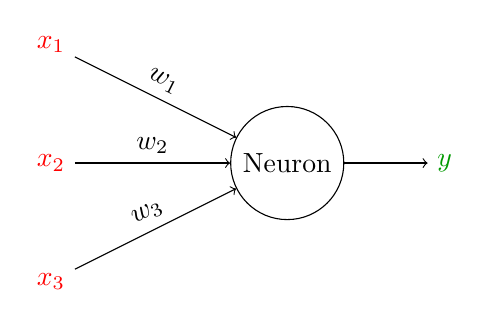
\begin{tikzpicture}
    \path (3,0) node [circle,draw](neuron){Neuron};
    \path[red] (0,1.5) node(x1){$x_1$} (0,0) node(x2){$x_2$} (0,-1.5) node(x3){$x_3$};
    \path[black!40!green] (5,0) node(y1){$y$};
    \draw[->] (x1) -- node[above,sloped]{$w_1$} (neuron);
    \draw[->] (x2) -- node[above,sloped]{$w_2$} (neuron);
    \draw[->] (x3) -- node[above,sloped]{$w_3$} (neuron);
    \draw[->] (neuron) -- (y1);
  \end{tikzpicture}
  \caption{ein Perzeptron mit drei Inputs}
  \label{fi:perzeptron}
\end{figure}

Fuer das Trainieren des Perzeptron existieren spezielle Verfahren, welche hier
aber nicht relevant sind. Das Gradientenverfahren kann naemlich nicht verwendet
werden. Der Grund dafuer sollte spaeter in Sektion (\ref{sec:kuenstlicheNeuronen}) einleuchtend werden.
\par\medskip
Nun stellt sich die Frage, was ein Perzeptron erlernen kann und wofuer es genutzt werden kann.
Das Perzeptron ist lediglich ein \textbf{Linearer Klassifikator} der Form
$y=w_1x_1+\cdots+w
_nx_n$.
Es kann die Features in zwei Klassen 0 oder 1 einordnen.
Ueberschreitet $y$ den Schwellenwert, werden die Features der Klasse 1 zugeordnet, sonst
der Klasse 0.
Jedoch muessen diese Klassen linear separierbar sein.
Das bedeutet, dass die Inputvektoren $\vec{x}$ durch eine Hyperebene trennbar
sein muessen.
Bei zwei Features (zwei Inputs) handelt es sich bei der Hyperebene um eine
Gerade welche die Vektoren auftrennt. Siehe Abbildung (\ref{fig:linearer_Klassifikator}).
Fuer drei Featuers ist es eine Ebene.
ZU ABSTRAKT -> BEISPIEL

Eine Funktionen, welche nicht linear separierbar ist (z.B\ XOR-Verknuepfungen),
kann von einem Perzeptron nicht erlernt werden.

\begin{figure}[h!]

  \caption{erfolgreiche lineare Separierung (links) und das Versagen bei XOR (rechts)}
  \label{fig:linearer_Klassifikator}
\end{figure}

\cite{wiki:perzeptron}

\subsubsection{Biologische Analogie}
SCHREIBEN
% Gewicht entscheidet ob inhibitorisch oder exaktorisch.
% Schwellenwert: Das Addieren eines Schwellenwerts  zur Netzeingabe verschiebt die gewichteten Eingaben. Die Bezeichnung bestimmt sich aus der Verwendung einer Schwellenwertfunktion als Aktivierungsfunktion, bei der das Neuron aktiviert wird, wenn der Schwellenwert überschritten ist. Die biologische Motivierung dabei ist das Schwellenpotential bei Nervenzellen. Mathematisch gesehen wird die Trennebene, die den Merkmalsraum auftrennt, durch einen Schwellenwert mit einer Translation verschoben.

% Hebbsche Lernregel

\subsubsection{Erweiterung der Kuenstlichen Neuronen}\label{sec:kuenstlicheNeuronen}
Ein Perzeptron ist, wie vorhin erklaert, nur in der Lage, lineare Klassifikationen
durchzufuehren. Um nun auch kompliziertere Probleme zu loesen, muss das Prinzip
ausgebaut werden. Ausserdem brauchen wir ein Kuenstliches Neuron, welches sich
besonders gut als Baustein fuer KNNs eignet.

\paragraph{Kuenstliche Neuronen im Allgemeinen}
Kuenstliche Neuronen sind immer so aufgebaut, dass sie einen oder mehrere Inputs
haben und einen einzigen Output. Zu jedem Input $x_i$ ist ein Gewicht
$w_{ji}$ assoziert. Zuerst wird die gewichtete Summe der Inputs $\tilde{z}$ gebildet.
Die Neigung $b$ wird ebenfalls draufaddiert, um $z$ zu erhalten. Nun muss
die sogennante Aktivierung $a$ gebildet werden. Sie entspricht dem Output des Neurons.
Die Aktivierung $a$ ist das Resultat der Aktivierungsfunktion $\varphi$ angewendet
auf $z$. $a = \varphi(z)$. Die verschiedenen Kuenstlichen Neuronen unterscheiden
sich fast nur in ihrer Aktivierungsfunktion.

\paragraph{Perzeptronen als Kuenstliche Neuronen}
Zuerst noch einmal ein Blick auf das Perzeptron in Betracht der Aktivierungsfunktion.
Ein wesentlicher Unterschied des Perzeptron gegenueber sonstigen Kuenstlichen
Neuronen, besteht darin, dass seine Inputs und Outputs nur binaere Werte
annehmen koennen. Um dieses Verhalten des Perzeptron zu erhalten,
muss eine Stufenfunktion als Aktivierungfunktion verwendet werden: die Heaviside-Funktion $\Theta$.
Sie hat einen einzigen Stufensprung bei $x=0$ vom Wert 0 auf 1. Siehe Abb. (\ref{fig:heaviside}).

\begin{figure}[h!]
  \begin{minipage}[h!]{0.5\textwidth}
    \begin{equation*}
      \varphi^{\text{hlim}}(z) = \Theta(z) =
      \begin{cases}
        1 & \quad \text{falls } z \geq 0\\
        0 & \quad \text{falls } z < 0
      \end{cases}
    \end{equation*}

  \end{minipage}
  \begin{minipage}[h!]{0.5\textwidth}
    \centering
    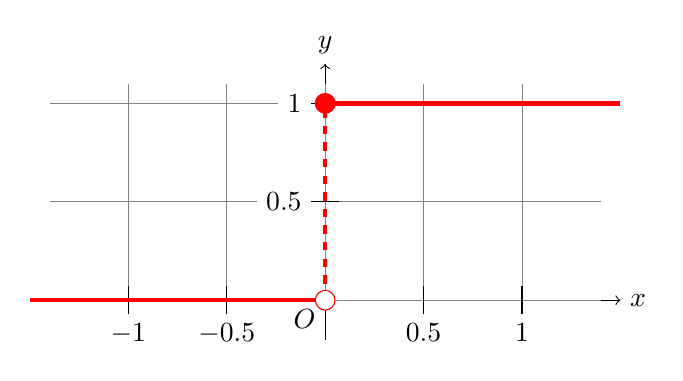
\begin{tikzpicture}[scale=2.5]

      \draw[->] (-1.5,0) -- (1.5,0) node[right] {$x$}; % x-axes
      \draw[->] (0,-0.2) -- (0,1.2) node [above] {$y$}; % y-axes
      \draw[style=help lines,step=0.5] (-1.4,0) grid (1.4, 1.1);

      \foreach \x in {-1,-0.5,0.5,1}
      \draw[shift={(\x,0)}] (0pt,2pt) -- (0pt,-2pt) node[below,fill=white] {$\x$};

      \foreach \y in {0.5,1}
      \draw[shift={(0,\y)}] (2pt,0pt) -- (-2pt,0pt) node[left,fill=white] {$\y$};

      \draw[shift={(0,0)}] (0pt,0pt) node[below left,fill=white] {$O$};

      \draw[red,ultra thick] (-1.5,0) -- (0,0); % 0-red
      \draw[red,ultra thick] (0,1) -- (1.5,1); % 1-red
      \draw[red,ultra thick,dashed] (0,0) -- (0,1); % y-red
      \draw[draw=red,fill=white] (0,0) circle (0.05);
      \draw[draw=red,fill=red] (0,1) circle (0.05);

    \end{tikzpicture}
  \end{minipage}

  \caption{die Definition und der Graph der Heaviside-Funktion $\Theta$}
  \label{fig:heaviside}
\end{figure}

\paragraph{Stueckweise lineare Neuronen}
Der naechste Schritt nach dem binaeren Perzeptron sind sogenannte stueckweise
lineare Neuronen.
Sie verwenden eine stueckweise lineare Aktivierungsfunktion. Diese bildet ein
beschraenktes Intervall linear ab. Die Werte ausserhalb werden auf die
konstanten Werte 0 oder 1 abbgebildet. Siehe Abb. (\ref{fig:stueckweiselinear}).
\par\medskip
Die Inputs koennen jetzt beliebige reelle Zahlen sein (vorzugsweise in der Naehe
von 0 und 1).
Ein KNN aus ausschliesslich linearen Neuronen ist ziemlich nutzlos, da jedliche Verkettung von
linearen Funktion auch durch eine einzige lineare Funktion dargestellt werden
koennte. Somit hat ein KNN gegenueber einem einzelnen Neuron keinen Mehrwert.
Ausserdem koennen mit diesen Neuron auch nur lineare Probleme geloest werden.

\begin{figure}[h!]
  \begin{minipage}[h!]{0.5\textwidth}
    \begin{equation*}
      \varphi^{\text{pwl}}(z) =
      \begin{cases}
        1 & \quad \text{falls } z > \frac{1}{2}\\
        z + \frac{1}{2} & \quad \text{falls } -\frac{1}{2} < z < \frac{1}{2}\\
        0 & \quad \text{falls } z < \frac{1}{2}
      \end{cases}
    \end{equation*}

  \end{minipage}
  \begin{minipage}[h!]{0.5\textwidth}
    \centering
    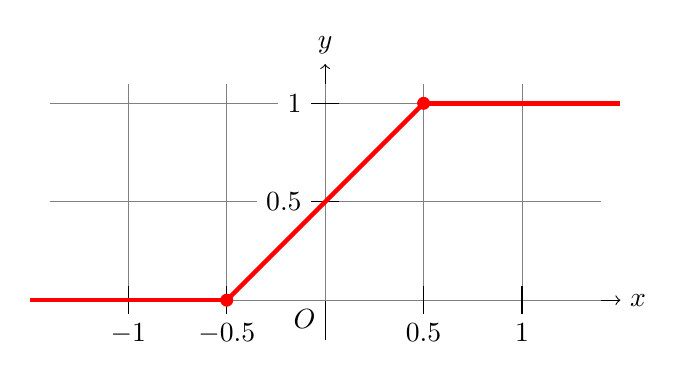
\begin{tikzpicture}[scale=2.5]

      \draw[->] (-1.5,0) -- (1.5,0) node[right] {$x$}; % x-axes
      \draw[->] (0,-0.2) -- (0,1.2) node [above] {$y$}; % y-axes
      \draw[style=help lines,step=0.5] (-1.4,0) grid (1.4, 1.1);

      \foreach \x in {-1,-0.5,0.5,1}
      \draw[shift={(\x,0)}] (0pt,2pt) -- (0pt,-2pt) node[below,fill=white] {$\x$};

      \foreach \y in {0.5,1}
      \draw[shift={(0,\y)}] (2pt,0pt) -- (-2pt,0pt) node[left,fill=white] {$\y$};

      \draw[shift={(0,0)}] (0pt,0pt) node[below left,fill=white] {$O$};

      \draw[red,ultra thick] (-1.5,0) -- (-0.5,0); % 0-red
      \draw[red,ultra thick] (0.5,1) -- (1.5,1); % 1-red
      \draw[red,ultra thick] (-0.5,0) -- (0.5,1); % d-red

      \draw[draw=red,fill=red] (-0.5,0) circle (0.03);
      \draw[draw=red,fill=red] (0.5,1) circle (0.03);


    \end{tikzpicture}
  \end{minipage}

  \caption{die Formel und der Graph einer stueckweisen linearen Funktion}
  \label{fig:stueckweiselinear}
\end{figure}


\paragraph{Sigmoide Neuronen}
Die logische naechste Erweiterung sind nicht-lineare Neuronen.
Ein sehr beliebter Kandidat dafuer sind Sigmoide Neuronen.
Den Namen haben sie von ihrer Aktivierungsfunktion: der Sigmoidfunktion $\sigma$.
Eine sehr wichtige Eigenschaft von ihr ist, dass sie - im Gegensatz zu den vorhin
genannten Aktivierungsfunktion - ueberall differenzierbar und strikt monoton
steigend ist. Erst fuer diese Aktivierungsfunktion, kann das Gradientenverfahren
angewendet werden und somit das KNN trainiert werden. Die anderen
Funktionen haben Stellen bei welchen die Ableitungsfunktion null
betraegt, somit kann das lokale Minimum nicht gefunden werden.
Nicht nur die Sigmoidfunktion erfuellt diese Bedingungen, sondern auch andere. Die Sigmoidfunktion wird
bevorzugt, da ihre Ableitung sehr simpel ist, siehe Abb. (\ref{fig:sigmoid}).
Die Nicht-linearitaet dieser Neuronen ermoeglicht ein Erlernen von deutlich komplexeren Sachverhalten.
Und wie spaeter in Sektion (\ref{sec:UAT}) erlautert, ist es moeglich mit der Kompostion von nicht-linearen
Funktionen jede belibige Funktion zu approximieren!
\par\medskip
Die Simgmoid-Funktion besitzt eine einzige Wendestelle bei $x=0$ und hat zwei Asymptoten, eine fuer $x \to -\infty$ mit $y=0$
und eine zweite fuer $x \to\infty$ mit $y=1$. Siehe Abb. (\ref{fig:sigmoid}).

\begin{figure}[h!]
  \begin{minipage}[h!]{0.5\textwidth}
    \begin{align*}
      \varphi^{\text{sig}}(z) &= \sigma(z) = \frac{1}{1 + e^{-z}}\\
      \sigma'(z)&=\sigma(z)(1-\sigma(z))
    \end{align*}
  \end{minipage}
  \begin{minipage}[h!]{0.5\textwidth}
    \centering
    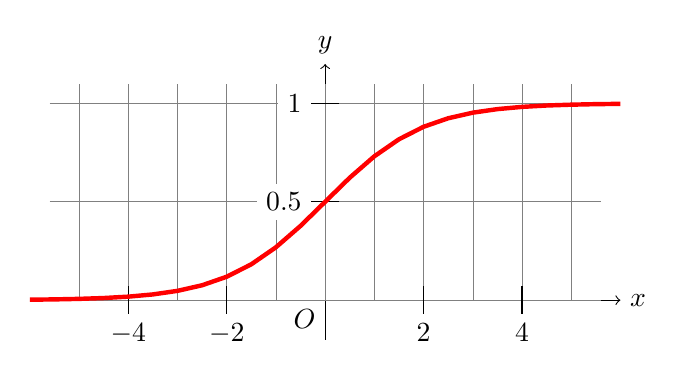
\begin{tikzpicture}[scale=2.5]

      \draw[->] (-1.5,0) -- (1.5,0) node[right] {$x$}; % x-axes
      \draw[->] (0,-0.2) -- (0,1.2) node [above] {$y$}; % y-axes
      \draw[style=help lines,ystep=0.5,xstep=0.25] (-1.4,0) grid (1.4, 1.1);

      \foreach \x/\xtext in {-1/-4,-0.5/-2,0.5/2,1/4}
      \draw[shift={(\x,0)}] (0pt,2pt) -- (0pt,-2pt) node[below,fill=white] {$\xtext$};

      \foreach \y in {0.5,1}
      \draw[shift={(0,\y)}] (2pt,0pt) -- (-2pt,0pt) node[left,fill=white] {$\y$};

      \draw[shift={(0,0)}] (0pt,0pt) node[below left,fill=white] {$O$};


      \draw[red,ultra thick,x=0.25cm] plot[domain=-6.0:6.0] (\x,{1/(1+exp(-\x)) });

    \end{tikzpicture}
  \end{minipage}

  \caption{die Formel und der Graph der Sigmoid-Funktion $\sigma$}
  \label{fig:sigmoid}
\end{figure}




\subsubsection{Topologie der Kuenstlichen Neuronalen Netzen}
Nun sollten diese Sigmoiden-Neuronen als Bausteine verwendet werden, um ein Kuenstliches
Neuronales Netz zu bilden. Dazu werden sie miteinander verbundet und bilden so ein Netz,
aehnlich wie ein Nervensystem.
Diese Neuronen sind in verschieden Schichten (engl.: Layers)
arangiert. Die erste ist die \textbf{Inputschicht}. Sie behinhalten die
Inputneuronen. Dies sind eigentlich keine richtigen
Neuronen sondern eher Platzhalter fuer ihren jeweiligen Inputwert $x_i$. Als letztes kommt die
\textbf{Outputschicht} mit den Outputneuronen, welche jeweils einen Outputwert $y_i$
besitzen. Dazwischen liegen die \textbf{Zwischenschichten} (engl.: Hiddenlayer). Von ihnen kann es
beliebig viele geben und in ihnen beliebig viele Neuronen.
Der Aufbau eines KNN bezeichnet man als \textbf{Topologie} des Netzes, es
handelt sich dabei um Hyperparameter.
\par\medskip
Jedes Neuron aus einer Schicht ist mit jedem Neuron aus der naechsten Schicht ueber
Verbindungen gekoppelt. Alle Verbindungen besitzten ein Gewicht analog zum
Perzeptron. Die Aktivierung, also der Output, eines Neurons wandert entlang den jeweiligen
Verbindung zu allen Neuronen der naechsten Schicht und dient als deren Input.
Die soeben beschriebe Art von KNN nennt man \textbf{Feedforward-Netz}, da alle Werte
ausschliesslich nach vorne propagiert werden.

\begin{figure}[h!]
  \centering
  \begin{tikzpicture}

    \tikzstyle{neuronstyle} = [inner sep=0,minimum size=1cm,circle,draw]

    \newcommand{\hiddenlayers}{2}
    \newcommand{\inputs}{4}
    \newcommand{\hiddens}{3}
    \newcommand{\outputs}{2}
    \newcommand{\radius}{1cm}
    \coordinate (spacev) at (0,-1.25cm);
    \coordinate (spaceh) at (2cm,0);
    \coordinate (spaceb) at (2cm,0);

    \foreach \j in {1,...,\inputs}
    \draw ($\j*(spacev)$) node[neuronstyle] (l0n\j) {$x_{\j}$};

    \foreach \l in {1,...,\hiddenlayers}
    \foreach \j in {1,...,\hiddens}
    \draw ($(spaceb) + \j*(spacev) + \l*(spaceh)$) node[neuronstyle] (l\l n\j) {$h_{\j}^{\l}$};

    \foreach \j in {1,...,\outputs}
    \draw ($2*(spaceb) + \hiddenlayers*(spaceh) + \j*(spacev)$) node[neuronstyle] (l3n\j) {$y_{\j}$};

    \foreach \j in {1,...,\inputs}
    \foreach \k in {1,...,\hiddens}
    \draw[->] (l0n\j) -- (l1n\k);

    \foreach \j in {1,...,\hiddens}
    \foreach \k in {1,...,\hiddens}
    \draw[->] (l1n\j) -- (l2n\k);

    \foreach \j in {1,...,\hiddens}
    \foreach \k in {1,...,\outputs}
    \draw[->] (l2n\j) -- (l3n\k);


  \end{tikzpicture}
  \label{fi:nn_layers}
  \caption{eine Darstellung der Schichtung eines KNN}
\end{figure}

\begin{figure}[h!]
  \centering
  \begin{tikzpicture}[
    % styles
    clear/.style={draw=none,fill=none},
    net/.style={matrix of nodes,nodes={draw,circle,inner sep=10pt},nodes in empty cell,column sep=2cm,row sep=-9pt},
    >=latex
    ]

    \matrix[net] (mat)
    {
      |[clear]| \parbox{1.3cm}{\centering Input\\layer}
      & |[clear]| \parbox{1.3cm}{\centering Hidden\\layer}
      & |[clear]| \parbox{1.3cm}{\centering Output \\layer} \\

      $\alpha_{0}^{0}$  & |[clear]|        & |[clear]| \\
      |[clear]|         & $\alpha_{0}^{1}$ & |[clear]| \\
      $\alpha_{1}^{0}$  & |[clear]|        & |[clear]| \\
      |[clear]|         & |[clear]|        & |[clear]| \phantom{$a_{0}^{0}$} \\
      $\alpha_{2}^{0}$  & $\alpha_{1}^{1}$ & $\alpha_{0}^{2}$ \\
      |[clear]|         & |[clear]|        & |[clear]|  \phantom{$a_{0}^{0}$} \\
      $\alpha_{3}^{0}$  & |[clear]|        & |[clear]| \\
      |[clear]|         & $\alpha_{2}^{1}$ & |[clear]| \\
      $\alpha_{4}^{0}$  & |[clear]|        & |[clear]| \\ 
    };

    % left most lines into input layers
    \foreach \ai in {2,4,...,10}
    \draw[<-] (mat-\ai-1) -- +(-2cm,0);

    % lines from a_{i}^{0} to each a_{j}^{1}
    \foreach \ai in {2,4,...,10} {
      \foreach \aii in {3,6,9}
      \draw[->] (mat-\ai-1) -- (mat-\aii-2);
    }

    % lines from a_{i}^{1} to a_{0}^{2}
    \foreach \ai in {3,6,9}
    \draw[->] (mat-\ai-2) -- (mat-6-3);
    
    % right most line with Output label
    \draw[->] (mat-6-3) -- node[above] {Output} +(2cm,0);
   }

  \end{tikzpicture}
  \caption{Test}
\end{figure}



\subsubsection{Vorwaertspropagierung}
Nachdem nun der Aufbau eines KNNs erklaert wurde, sollte nun die mathematische Funktionsweise
des Modells erklaert werden. Hierfuer muessen einige Konventionen zur
Bezeichnung der Teile eines KNNs getroffen werden:

\begin{itemize}

\item{$n_j^l$ bezeichnet das $j$-te Neuron in der $l$-ten Schicht.}
\item{$z_j^l$ ist die gewichtete Summe der Inputs des $j$-ten Neuron in der $l$-ten Schicht.}
\item{$a_j^l$ ist die Aktivierung des $j$-ten Neurons in der $l$-ten Schicht.}
\item{$b_j^l$ ist die Neigung des $j$-ten Neuron in der $l$-ten Schicht.}
\item{$w_{j,k}^l$ ist das Gewicht der Verbindung vom $k$-ten Neuron
    in der ($l-1$)-ten Schicht zum $j$-ten Neuron in der $l$-ten Schicht (man
    beachte die Reihenfolge)
    \footnote{
      Diese Konvention scheint auf den ersten Blick unintuitiv, macht jedoch
      Sinn fuer die spaeteren mathematischen Operationen mit Matrizen in Sektion
      (\ref{sec:backpropagation}).
    }.}

\item{$L$ soll die gesamte Anzahl der Schichten sein.}

\item{$N_l$ ist die Anzahl Neuronen in der $l$-ten Schicht.} 

\item{$\varphi$ ist die gewaehlte Aktivierungsfunktion (grundsaetzlich ist diese
    immer die Sigmoidfunktion $\sigma$).}

\end{itemize}

\begin{figure}[h!]
  \centering
  \begin{tikzpicture}

    \newcommand{\hiddenlayers}{3}
    \newcommand{\inputs}{4}
    \newcommand{\hiddens}{3}
    \newcommand{\outputs}{2}
    \newcommand{\radius}{1cm}
    \coordinate (spacev) at (0,-1cm);
    \coordinate (spaceh) at (1cm,0);
    \coordinate (spaceb) at (2cm,0);

    \foreach \j in {1,...,\inputs}
    \draw ($\j*(spacev)$) node[inner sep=0,minimum size=1cm,circle,draw] (l0n\j) {$a_{\j}^0$};

    % \foreach \l in {1,...,\hiddenlayers}
    % \foreach \j in {1,...,\hiddens}
    % \draw ($\j*(spacev) + \l*(spaceh) + (spaceb)$) node[inner sep=0,minimum size=1cm,circle,draw] (l\ln\j) {$h_{\j}^{\l}$};

    % \foreach \j in {1,...,\outputs}
    % \draw ($\j*(spacev) + 2*(spaceb) + \hiddenlayers*(spaceh)$) node[inner sep=0,minimum size=1cm,circle,draw] (l8n\j) {$y_{\j}$};

    % \foreach \j in {1,...,\inputs}
    % \foreach \k in {1,...,\hiddens}
    % \draw[->] (n:0:\j) -- (n:1:\k);

    % \draw[->] (l0n1) -- (l1n1);

  \end{tikzpicture}
  \label{fi:nn_layers}
  \caption{Abbildung zum Verstaentniss der Nomenklatur}
\end{figure}

\par\bigskip
Die Vorwaertspropagierung beginnt bei den Inputneuronen, welche mit ihren
Inputwerten befuettert werden. Diese werden, um eine kohaerente Nomenklatur zu haben,
gleich wie die Aktivierungen der anderen Neuronen mit $a_j^0$ bezeichnet, wobei
$j$ der Index des Neurons ist.\par
Die restlichen Aktivierungen der Neuronen werden rekursiv anhand der
Aktivierungen der voherigen Schicht berechnet. Und zwar folgendermassen:\par
Zuerst laueft eine Summe ueber alle Neuronen $n_k^{l-1}$ der voherigen Schicht
($l-1$). Dabei wird die gewichtete Summe der Aktivierungen $a_k^{l-1}$ mit den
assozierten Gewichten $w_{j,k}^l$ gebildet, dabei ist das Gewicht jenes, welches das
$k$-te Neuron der ($l-1$)-ten Schicht mit dem $j$-ten Neuron der $l$-ten Schicht verbindet.
Zu der gewichteten Summe gehoert auch die jeweilige Neigung $b_j^l$, welche
dazuaddiert wird. Diese gewichtete Summe wird mit $z_j^l$ bezeichnet.

\begin{equation}\label{eq:gewichtete_summe_normal}
  z_j^l = \sum_{k=1}^{N_l} w_{j,k}^l a_k^{l-1} + b_j^l
\end{equation}

Auf diese Summe wird dann die Aktivierungsfunktion $\varphi$ angewandt.
Das ist dann die Aktivierung des Neurons.

\begin{equation}\label{eq:aktivierung_normal}
  a_j^l = \varphi\left(\sum_{k=1}^{N_l} w_{j,k}^l a_k^{l-1} + b_j^l \right) = \varphi \left( z_j^l \right)
\end{equation}
\par\bigskip
Da KNNs weit verbreitet sind in der Bilderkennung und Spracherkennung, ist es
nicht unueblich, dass diese sehr viele Neuronen und Verbindungen (ueber 100'000) besitzen.
Um hierbei nicht den Ueberblick zu verlieren und um nicht in den Indizes zu
ertrinken, greift man auf \textbf{Lineare Algebra} zurueck. Man verwendet
Matrizen und Vektoren um die vielen Variabeln zusammen zu fassen.
Ausserdem koennen Computer deutlich schneller Matrixoperationen ausfuehren, als
alle Zahlen einzeln zu verrechnen. Dies beschleunigt das Training der Modelle um
ein Vielfaches. Dies wird spaeter in Sektion
(\ref{sec:tensorflow}) noch mehr erlauetert.
\par\medskip
Um nun lineare Algebra ins Spiel zu bringen, wird eine \textbf{Gewichtsmatrix}
$\mat{W}^l$ fuer jede Schicht $l$ definiert.
Die Eintraege dieser Matrix sind einfach die Gewichte welche zu den Neuronen der
$l$-ten Schicht verlaufen. Das heisst der Eintrag in der $j$-ten Zeile und in
der $k$-ten Spalte ist $w_{j,k}^l$ (Siehe Gl. (\ref{eq:gewichtsmatrix})). Ebenfalls werden alle Neigung $b_j^l$ in
einer Schicht $l$ zu einem Vektor $\vec{b}^l$ zusammmen gefasst. Und zu guter
Letzt wird ein Aktivierungsvektor $\vec{a}^l$, welcher alle Aktiverungen $a_j^l$
einer Schicht $l$ einfaengt.

\begin{equation}\label{eq:gewichtsmatrix}
  \mat{W}^l =
  \begin{pmatrix}
    w_{1,1}^l & w_{1,2}^l & \cdots & w_{1,n}^l \\[0.3em]
    w_{2,1}^l & w_{2,2}^l & \cdots & w_{2,n}^l \\[0.3em]
    \vdots & \vdots & \ddots & \vdots \\[0.3em]
    w_{m,1}^l & w_{m,2}^l & \cdots & w_{m,n}^l
  \end{pmatrix}
\end{equation}

Um nun Gleichung (\ref{eq:aktivierung_normal}) in der Matrixform zu schreiben,
muss noch die Vektoriesierung einer Funktion eingefuehrt werden.
\par\medskip

\begin{defbox}{Vektorisierung einer Funktion}
  Die Vektoriserung einer Funktion $f$, geschrieben als $f[\vec{v}]$ ist eine neue Funktion, welche die Funktion $f$ auf jede Vektorkomponente anwendet und einen neuen Vektor als Rueckgabewert hat.
  \begin{equation*}
    f[\vec{v}]=
    \begin{pmatrix}
      f(v_1)\\
      \vdots \\
      f(v_n)\\
    \end{pmatrix}
  \end{equation*}
\end{defbox}

\par\medskip

Nun kann die Matrixschreibweise eingefuehrt werden (siehe Gleichung (\ref{eq:aktivierung_matrix})).\par
Zuerst wird eine Matrixmultiplikation der Gewichtsmatrix $\mat{W}^l$ mit dem
Aktivierungsvektor $\vec{a}^{l-1}$ der vorherigen Schicht durchgefuehrt. Darauf
wird der Neigunsvektor addiert. Und zu guter Letzt wird die vektorisierte
Aktivierungsfunktion $\varphi$ angewandt.
\begin{equation}\label{eq:aktivierung_matrix}
  \vec{z}^{\,l} = \mathbf{W}^{\,l} \vec{a}^{\,l-1} + \vec{b}^{\,l}
\end{equation}
\par
\begin{equation}\label{eq:aktivierung_matrix}
  \vec{a}^{\,l} = \varphi \left[\mat{W}^{\,l} \vec{a}^{\,l-1} + \vec{b}^{\,l} \right] = \varphi \left[ \vec{z}^l \right]
\end{equation}


\subsubsection{Gewichte und Neigungen initalisieren*}

\subsubsection{Rueckwaertspropagierung}\label{sec:backpropagation}
Das Gradientenverfahren fuer KNN bezeichnet man als
\textbf{Rueckwaertspropagierung} (engl.: Backpropagation).

Das Ziel dieses Algorithmus ist es die beiden Partiellen Ableitungen
$\frac{\partial C}{\partial w_{j,k}^l}$ und $\frac{\partial C}{\partial b_j^l}$
zu bestimmen. Hierfuer ist es sinnvoll eine Zwischenwert, welchen wir Fehler
$\delta_j^l$ nennen.

\par\medskip
\begin{defbox}{Hadamard-Produkt}
  Das Hadamard-Produkt ist ein spezielles Produkt zweier gleichgrossen Matrizen.
  Die resultierende Matrix ergibt sich aus der elementweisen Multiplikation der Ausgangsmatrizen.

  \begin{minipage}{0.5\textwidth}
    \begin{equation*}
      \mat{A} \odot \mat{B} =
      \begin{pmatrix}
        a_{1,1} b_{1,1} & \cdots & a_{1,n} b_{1,n} \\[0.3em]
        \vdots & \ddots & \vdots \\[0.3em]
        a_{m,1} b_{m,1} & \cdots & a_{m,n} b_{m,n} \\[0.3em]
      \end{pmatrix}
      \in \mathbb{R}^{m \times n}
    \end{equation*}
  \end{minipage}
  % 
  \begin{minipage}{0.5\textwidth}
    \begin{equation*}
      \vec{v} \odot \vec{w} =
      \begin{pmatrix}
        v_1 w_1 \\
        \vdots \\
        v_n w_n
      \end{pmatrix}
    \end{equation*}

  \end{minipage}
\end{defbox}
\par\medskip

\begin{equation}
  \delta_j^l \coloneqq \frac{\partial C}{\partial z_j^l}
\end{equation}

Viel Kettenregel.

\begin{equation}
  \frac{\partial C}{\partial w_{j,k}} = \frac{\partial C}{\partial a_k} \frac{\partial a_k}{\partial z_k} \frac{\partial z_k}{\partial w_{j,k}}
\end{equation}

Die vier magischen Gleichungen:

Der Fehler in der Outputschicht
\begin{equation}\tag{BP1}
  \delta_j^L = \frac{\partial C}{\partial a_j^L} \sigma'(z_j^L)
\end{equation}

Matrixform
\begin{equation}\tag{BP1a}
  \delta^L = \nabla_aC \odot \sigma'(z^L)
\end{equation}
Das tiefgestellte $_a$ des Nablas, gibt an, dass es sich um den Gradienten mit den partiellen
Ableitungen bezueglich den Aktivierungen $a$ handelt.

Fehler anhand des Fehlers der naechsten Schicht
\begin{equation}\tag{BP2}
  \delta^l = (\trs{(w^{l+1})} \delta^{l+1}) \odot \sigma'(z^l)
\end{equation}

\begin{equation}\tag{BP3}
  \frac{\partial C}{\partial b_j^l} = \delta_j^l
\end{equation}

\begin{equation}\tag{BP4}
  \frac{\partial C}{\partial w_{j,k}^l} = a_k^{l-1} \delta_j^l
\end{equation}



\subsubsection{Universal Approximation Theorem}\label{sec:UAT}
Neural Network kann alles erlernen

\subsection{Autoencoder und Convolutional KNN}
\subsubsection{Autoencoder}
\subsubsection{Bedeutung von Autoencodern}
\paragraph{Datenkompression}
~Hauptkomponentenanalyse und Dimensionalitatsreduktion
\paragraph{Datengenerierung}
\paragraph{Eigenschaften erkennen}

\subsubsection{Convolutional KNN}

\subsubsection{Variational Autoencoder?}
\subsubsection{Detangled Autoencoder?}


\end{document}


%%% Local Variables:
%%% mode: latex
%%% TeX-master: "../main"
%%% End:
